%!TEX TS-program = xelatex
%!TEX encoding = UTF-8 Unicode
\documentclass[a4paper, 12pt, oneside]{book}

\usepackage{cite}
%\usepackage{chapterbib}
%The chapterbib package facilitates multiple bibliographies in a LATEX document
\usepackage[hyphens]{url}
%Verbatim with URL-sensitive line breaks.
\usepackage[colorlinks=true,linkcolor=black,citecolor=black,filecolor=blue,urlcolor=blue,unicode]{hyperref}
%The hyperref package is used to handle cross-referencing commands in LaTeX to produce hypertext links in the document. The package provides backends for the \special set defined for HyperTeX DVI processors; for embedded pdfmark commands for processing by Acrobat Distiller (dvips and Y&Y��s dvipsone); for Y&Y��s dviwindo; for PDF control within pdfTeX and dvipdfm; for TeX4ht; and for VTeX��s pdf and HTML backends.

\usepackage{verbatim}
%The verbatim environment  simply reproduces every character you input, including all  s p a c e s!
\usepackage{color}
%you can set the color of the font of the text, and set the background color of the page.
\usepackage[dvipsnames]{xcolor}
%xecolor package is a simple package which defines about 140 different colors by XeTeX's font
\usepackage{graphicx}
%Standard LaTeX graphics.
%\usepackage{array}
%The array environment is used to make a table of information, with column alignment (left, center, or right) and optional vertical lines separating the columns.
%\usepackage{gensymb}
%Provides generic commands \degree, \celsius, \perthousand, \micro and \ohm which work both in text and maths mode.
\usepackage{indentfirst}
%Make the first line of all sections etc., be indented by the usual paragraph indentation. This should work with all the standard document classes. This minimalist package is part of the "tools" bundle in the LaTeX required distribution.
%\usepackage{algorithm}
%\usepackage{algpseudocode}
%A suite of tools for typesetting algorithms in pseudo-code. The algorithmicx package provides many possibilities to customize the layout of algorithms. You can use one of the predefined layouts (pseudocode, pascal and c and others), with or without modifications, or you can define a completely new layout for your specific needs.
\usepackage{enumitem}
%Control layout of itemize, enumerate, description.  It supersedes both enumerate and mdwlist (providing well- structured replacements for all their funtionality), and in addition provides functions to compute the layout of labels, and to 'clone' the standard environments, to create new environments with counters of their own.
\usepackage{mfirstuc}
%\makefirstuc{�qstuff �r} This makes the first object of �qstuff �r uppercase unless �qstuff �r starts with a con- trol sequence followed by a non-empty group, in which case the first object in the group is converted to uppercase.
\usepackage{fancyvrb}
%This package provides very sophisticated facilities for reading and writing ver- batim TEX code.
\usepackage{amsfonts}
%TeX fonts from the American Mathematical Society.
\usepackage{ifmtarg}
%If-then-else command for processing potentially empty arguments.
\usepackage{amsmath}
%The amsmath package is a LATEX package that provides miscellaneous enhance- ments for improving the information structure and printed output of documents that contain mathematical formulas.
\usepackage{amssymb}
% Math symbols
\usepackage[mathcal]{euscript}
%This file sets up some font shape definitions to use the Euler script symbols in math mode.
\usepackage[notbib]{tocbibind}
%Add (or disable) bibliography/index/contents to Table of Contents.
\usepackage{rotating}
%Rotation tools, including rotated full-page floats.
%\usepackage{hhline}
%The command \hhline produces a line like \hline, or a double line like \hline\hline, except for its interaction with vertical lines. The command takes a preamble (rather like the preamble of a tabular environment), and this specifies whether there are to be one or two horizontal lines, and what happens when the horizontal line meets a vertical one. The package is part of the tools bundle in the LaTeX required distribution.
\usepackage{wallpaper}
%Easy addition of wallpapers (background images) to LaTeX documents, including tiling.
\usepackage{pdfpages}
%Include PDF documents in LaTeX.
\usepackage{pst-fractal,pst-exa}
% The package will draw the Julia and Mandelbrot sets, the Sierpinski triangle, Koch flake, and Apollonius Circle as well as fractal trees (which need not be balanced) with a variety of different parameters (including varying numbers of iterations).

%Define \XeTeX \XeLaTeX command
\def\reflect#1{{\setbox0=\hbox{#1}\rlap{\kern0.5\wd0
 \special{x:gsave}\special{x:scale -1 1}}\box0 \special{x:grestore}}}
\def\XeLaTeX{\leavevmode
 \setbox0=\hbox{X\lower.5ex\hbox{\kern-.15em\reflect{E}}\kern-.08em\LaTeX}%
 \dp0=0pt\ht0=0pt\box0}
 \def\XeTeX{\leavevmode
 \setbox0=\hbox{X\lower.5ex\hbox{\kern-.15em\reflect{E}}\kern-.08em\TeX}%
 \dp0=0pt\ht0=0pt\box0}

% \usepackage[none]{hyphenat}  %hyphenation package

% Start Declare physics symbols
\newcommand{\gv}[1]{\ensuremath{\mbox{\boldmath$ #1 $}}} 
\newcommand{\grad}[1]{\gv{\nabla} #1} % for gradient
\let\divsymb=\div % rename builtin command \div to \divsymb
\renewcommand{\div}[1]{\gv{\nabla} \cdot #1} % for divergence
\newcommand{\curl}[1]{\gv{\nabla} \times #1} % for curl
\let\baraccent=\= % rename builtin command \= to \baraccent
\renewcommand{\=}[1]{\stackrel{#1}{=}} % for putting numbers above =
%end Declare

\usepackage{booktabs}				% ����u��
\usepackage{tabularx}
%tabularx, is defined, which takes the same arguments as tabular*, but modifies the widths of certain columns, rather than the inter column space, to set a table with the requested total width. The columns that may stretch are marked with the new token X in the preamble argument. This package requires the array package. The package is part of the tools bundle in the LaTeX required distribution.
%\usepackage{lmodern}
%The Latin Modern family of fonts consists of 72 text fonts and 20 mathematics fonts, and is based on the Computer Modern fonts released into public domain by AMS (copyright c 1997 AMS).
%\font\lmr="[lmroman10-regular]"

%\usepackage{listings}
%Typeset source code listings using LaTeX.
%\usepackage{textcomp}
%provide many text symbols (such as baht, bullet, copyright, musicalnote, onequarter, section, and yen)

\usepackage{amsthm}
%The package facilitates the kind of theorem setup typically needed in American Mathematical Society publications. The package offers the theorem setup of the AMS document classes (amsart, amsbook, etc.) encapsulated in LaTeX package form so that it can be used with other document classes. Amsthm is part of the (required) AMS-LaTeX distribution, so should be present in any LaTeX distribution.
\newtheorem{mydef-no-caption}{Definition}
\newenvironment{mydef}[1][]%
	{\begin{mydef-no-caption}{\ifnotmtarg{#1}{\textnormal{(\textbf{#1})}~}}}%
	{\end{mydef-no-caption}}

\usepackage{numprint}
%Print numbers with separators and exponent if necessary.
\npthousandsep{,}
\npthousandthpartsep{}
\npdecimalsign{.}

\usepackage{multirow}
%Create tabular cells spanning multiple rows.

\usepackage{ntu}
%NTU thesis style file
\hypersetup{
	pdfauthor={\authorEN{}},
	pdftitle={\titleEN{}},
	pdfsubject={NTU Thesis}
}

\usepackage{setspace}
%Set space between lines.

\usepackage[absolute]{textpos}
%Place boxes at arbitrary positions on the LaTeX page.
\lstdefinestyle{nonumbers}{numbers=none}
\textblockorigin{0mm}{0mm}

\setcounter{tocdepth}{2}

\pagestyle{plain}

\usepackage{CJKnumb}
\usepackage{titletoc}					% 目錄修改套件
\usepackage{titlesec} 				% 美化章節標題套件

% === 圖表相關設定 ===

\graphicspath{{images/}} 			% 設定圖形路徑

\newcommand{\loflabel}{圖}
\newcommand{\lotlabel}{表}
\renewcommand\figurename{\loflabel}
\renewcommand\tablename{\lotlabel}
\setlength{\abovecaptionskip}{10pt} % 修改圖表標題和圖表內容的間距
\setlength{\belowcaptionskip}{10pt} % 修改圖表標題和圖表內容的間距

% === 自訂指令 ===
\renewcommand\contentsname{目錄}
\renewcommand\listfigurename{圖目錄}
\renewcommand\listtablename{表目錄}
\renewcommand\bibname{參考文獻}

\setlength{\parindent}{22pt}  	% 設定縮排

\newboolean{isAppendix}
\setboolean{isAppendix}{false}


% === 目錄標題 (配合 titletoc) ===
\titlecontents{chapter}[0em]{\fontsize{12}{18}\selectfont}
  {\hspace{3.5em}\contentslabel[第\CJKnumber{\thecontentslabel}章]{3.5em}}
  {}{\hspace{0.5em}\titlerule*{.}\contentspage}

\titlecontents{section}
[3.5em]
{\fontsize{12}{18}\selectfont}
{\contentslabel{2em}}
{}{\hspace{0.5em}\titlerule*{.} \contentspage}

\titlecontents{subsection}
[6.5em]
{\fontsize{12}{18}\selectfont}
{\contentslabel{3em}}
{}{\hspace{0.5em}\titlerule*{.} \contentspage}

% === 章節標題 (配合 titlesec) ===
\titleformat{\chapter}[display]
	{\bf\Large}
	{\filleft 第\,\CJKnumber{\thechapter}\,章}
	{1ex}
	{\huge\titlerule
	 \vspace{2ex}%
	 \filright}
	[\vspace{2ex}%
	 \titlerule]


\begin{document}

%----------- hyphenation  -----------
%\righthyphenmin=10  % Best hyphenation parameter

%----------- watermark -----------
\CenterWallPaper{0.174}{watermark.pdf}
\setlength{\wpXoffset}{6.1725cm}
\setlength{\wpYoffset}{10.5225cm}

%----------- cover page -----------
\maketitle

%----------- side page, used for printing on spline -----------
\makeside


\frontmatter
%----------- generate the certification page by LaTeX -----------
\makecertification
%----------- includepdf by using package pdfpages -----------
%\addcontentsline{toc}{chapter}{口試委員會審定書}
%\includepdf[pages={1}]{cert.pdf}

\onehalfspacing
\begin{acknowledgementsCH}
 這裡將簡單介紹如何利用\LaTeX\ 來編輯你的畢業論文,若不知道\LaTeX\ 是什麼或是沒有概念的話,建議你可以簡單看過放在此資料夾裡的\href{run:./latex123.pdf}{李果正-大家來學\LaTeX}前四章內容,在下載適合的\LaTeX\ 整合發行套件之後(請看第~\ref{it:download}項),可以嘗試用剛安裝好的\LaTeX\ 編輯器來編譯\href{run:./thesis.tex}{thesis.tex}這份文件,編譯的方法可以看下面第~\ref{it:comp}項的介紹,若編譯成功,所編譯出來的thesis.pdf文件的應該會跟此demo.pdf文件一模一樣,而且沒有任何問號符號,走到這一步的話,就差不多可以開始邊學習\LaTeX\ 邊編輯你的畢業論文了!基本上會使用到的指令都包含在論文的的各章節裡,怎麼在論文裡寫公式或是放圖之類的就自行看tex檔學吧。如果有任何問題或建議可以來信與我討論,我的信箱是\href{mailto:dran31545@gmail.com}{dran31545@gmail.com},或是到此範本\href{http://code.google.com/p/ntu-thesis-latex-template/}{Google Project}裡面的\href{http://code.google.com/p/ntu-thesis-latex-template/issues/list}{Issues}貼上你的問題與建議,我會盡我所能更新此範本,也歡迎大家自行重製、改良此範本並散布給他人,祝大家順利畢業!\\\\
 要編輯致謝請打開\href{run:./acknowledgementsCH.tex}{acknowledgementsCH.tex}\\
 \begin{enumerate}[leftmargin=0pt, topsep=0pt, itemsep=0pt, label=\Roman{*}.]
\item 此範本參考並修改自下列網站的資料:
\begin{enumerate}[topsep=0pt, itemsep=0pt, label=$\bullet$]
    \item \href{http://www.csie.ntu.edu.tw/~tzhuan/www/resources/ntu/}{如何用 LaTeX 排版臺灣大學碩士論文}\\
    \textemdash 台灣大學論文\LaTeX\ 樣版原創者\href{http://www.csie.ntu.edu.tw/~tzhuan/www/}{黃子桓}的教學網頁
    \item \href{http://www.hitripod.com/blog/2012/05/latex-thesis-template-quick-reference/}{LaTeX 常用語法及論文範本}\\
    \textemdash \href{http://www.hitripod.com/blog/}{Hitripod}所修改的範本,這裡參考了許多他所寫的格式和內容
    \item \href{http://www.cc.ntu.edu.tw/chinese/epaper/0014/20100920_1404.htm}{使用LaTeX做出精美的論文}
    \item \href{http://www.hitripod.com/blog/2011/04/xetex-chinese-font-cjk-latex/}{XeTeX:解決 LaTeX 惱人的中文字型問題}
    \item \href{http://code.google.com/p/ntuthesis/}{台灣大學碩士、博士論文的Latex模板}\\
\end{enumerate}
\item 幾個有用的參考資料及網路資源:
\begin{enumerate}[topsep=0pt, itemsep=0pt, label=$\bullet$]
    \item \href{run:./latex123.pdf}{李果正-大家來學\LaTeX}\textemdash 建議先看完前四章
    \item \href{http://en.wikibooks.org/wiki/LaTeX}{WIKIBOOKS-\LaTeX}\textemdash 好用的線上工具書
    \item \href{run:./Working_with_a_bib_file_using_Jabref.pdf}{Working with a .bib file using JabRef}
    \item \href{run:./Fi087_S.pdf}{Using BibDesk - A short tutorial}
    \item \href{http://www.dfcd.net/articles/latex/latex.html}{LaTeX for Physicists}\\
\end{enumerate}
\item 下載\LaTeX\ 整合發行套件,可參考\href{http://www.tug.org/texcollection/}{TeX Collection}:\label{it:download}
 \begin{enumerate}[topsep=0pt, itemsep=0pt, label=\arabic{*}.]
     \item \href{http://www.tug.org/mactex/}{MacTeX}: For \textcolor{Green}{\textbf{MacOSX}},下載\href{http://mirror.ctan.org/systems/mac/mactex/MacTeX.pkg}{MacTeX.pkg}
     \item \href{http://www.tug.org/protext/}{ProTeXt}: For \textcolor{Green}{\textbf{Windows}},下載\href{ftp://ftp.fernuni-hagen.de/pub/windows/win32/ProTeXt/}{ISO file}
     \item \href{http://www.tug.org/texlive/}{TeX Live}: For \textcolor{Green}{\textbf{GNU/Linux}} and \textcolor{Green}{\textbf{MacOSX}}, and \textcolor{Green}{\textbf{Windows}},下載\href{http://www.tug.org/texlive/acquire-iso.html}{ISO file}
     \item \href{http://ctan.org/}{CTAN}: The Comprehensive TeX Archive Network.\\
 \end{enumerate}

\item 好用的程式:
 \begin{enumerate}[topsep=0pt, itemsep=0pt, label=$\bullet$]
    \item 文獻管理系統:
        \begin{enumerate}[topsep=0pt, itemsep=0pt, label=\arabic{*}.]
         \item \href{http://jabref.sourceforge.net/}{JabRef}\\
                     可參考\href{run:./Working_with_a_bib_file_using_Jabref.pdf}{Working with a .bib file using JabRef}或是\href{https://www.google.com/search?q=jabref}{Google}及\href{http://www.youtube.com/results?search_query=jabref}{YouTube}
         \item \href{http://bibdesk.sourceforge.net/}{BibDesk} (For Mac)\\
                     可參考\href{run:./Fi087_S.pdf}{Using BibDesk - A short tutorial}或是\href{https://www.google.com/search?q=bibdesk}{Google}及\href{http://www.youtube.com/results?search_query=bibdesk}{YouTube}
         \end{enumerate}
         \item 方程式編輯器:\href{https://chrome.google.com/webstore/detail/dinfmiceliiomokeofbocegmacmagjhe?hl=zh-TW}{Daum Equation Editor} (Chrome App,必須使用Google瀏覽器)\\
 \end{enumerate} 
\item 編譯流程:\label{it:comp}
\begin{enumerate}[topsep=0pt, itemsep=0pt, label=\arabic{*}.]
    \item \texttt{xelatex thesis}\\ 對thesis.tex進行第一次XeLaTeX編譯,產生thesis.pdf以其他檔案
    \item \texttt{bibtex thesis}\\ 對thesis.tex進行BibTeX編譯,產生bbl檔以及blg檔
    \item \texttt{xelatex thesis}\\ 對thesis.tex進行第二次XeLaTeX編譯,產生目錄、圖表連結及參考文獻
    \item \texttt{xelatex thesis}\\ 對thesis.tex進行第三次XeLaTeX編譯,產生參考文獻連結,完成編譯
\end{enumerate} 
    \textcolor{Red}{注意!}此範本使用cite套件,可依據你利用文獻管理系統所整理好的\href{run:./thesisbib.bib}{thesisbib.bib}檔在論文最後產生參考文獻頁面,若你的系所規定要在每個章節的後面產生參考文獻,則可以用chapterbib套件,來對每個有附參考文獻的章節tex檔進行一次BibTeX編譯產生bbl檔,如範例的\href{run:./introduction.tex}{introduction.tex}、\href{run:./THM.tex}{THM.tex}和\href{run:./EXP.tex}{EXP.tex},如果有這需要請把\href{run:./thesis.tex}{thesis.tex}檔裡使用cite套件的指令利用註解符號\texttt{\%}來取消使用cite套件,並刪去出現在使用chapterbib套件指令前面的註解符號\texttt{\%}來啟動使用chapterbib套件
    \begin{verbatim}
\usepackage{cite}
%\usepackage{chapterbib}
改成
%\usepackage{cite}
\usepackage{chapterbib}
    \end{verbatim}
    再來利用註解符號\texttt{\%}取消會把參考文獻放在論文最後的指令
    \begin{verbatim}
\bibliographystyle{unsrt}
\addcontentsline{toc}{chapter}{\bibname}
\bibliography{thesisbib}
改成
%\bibliographystyle{unsrt}
%\addcontentsline{toc}{chapter}{\bibname}
%\bibliography{thesisbib}
    \end{verbatim}
    再把用來輸入章節檔案的\texttt{\textbackslash input}指令改成\texttt{\textbackslash include}指令
     \begin{verbatim}
\input{introduction}  =>  \include{introduction}
\input{THM}           =>  \include{THM}
\input{EXP}           =>  \include{EXP}
     \end{verbatim}
    最後記得在每個有附參考文獻的章節加上產生參考文獻的指令,即在\href{run:./introduction.tex}{introduction.tex}、\href{run:./THM.tex}{THM.tex}和\href{run:./EXP.tex}{EXP.tex}三個檔案裡最後啟動下面兩行指令
     \begin{verbatim}
%\bibliographystyle{unsrt} => \bibliographystyle{unsrt}
%\bibliography{thesisbib}  =>  \bibliography{thesisbib}
     \end{verbatim}
    而編譯時則需要對有附參考文獻的\href{run:./introduction.tex}{introduction.tex}、\href{run:./THM.tex}{THM.tex}和\href{run:./EXP.tex}{EXP.tex}各做一次BibTeX 編譯,編譯流程如下
    \begin{enumerate}[topsep=0pt, itemsep=0pt, label=\arabic{*}.]
    \item \texttt{xelatex thesis}\\ 對thesis.tex進行第一次XeLaTeX編譯,產生thesis.pdf及其他檔案
    \item \texttt{bibtex introduction}\\ 對introduction.tex進行BibTeX編譯,產生bbl檔以及blg檔
    \item \texttt{bibtex THM}\\ 對THM.tex進行BibTeX編譯,產生bbl檔以及blg檔
    \item \texttt{bibtex EXP}\\ 對EXP.tex進行BibTeX編譯,產生bbl檔以及blg檔
    \item \texttt{xelatex thesis}\\ 對thesis.tex進行第二次XeLaTeX編譯,產生目錄、圖表連結及參考文獻
    \item \texttt{xelatex thesis}\\ 對thesis.tex進行第三次XeLaTeX編譯,產生參考文獻連結,完成編譯\\
\end{enumerate} 
\item 補充說明與注意事項:
\begin{enumerate}[topsep=0pt, itemsep=0pt, label=$\bullet$]
    \item 口試委員會審定書:\\
    請到台大圖書館網頁的\href{http://etds.lib.ntu.edu.tw/etdsystem/submit/submitLogin}{電子論文服務}下載\href{http://gra103.aca.ntu.edu.tw/gra2007/gra/tienn/\%E5\%AD\%B8\%E4\%BD\%8D\%E8\%80\%83\%E8\%A9\%A6\%E8\%A1\%A8\%E5\%86\%8A/THESISSAMPLE.DOC}{論文格式範本},並修改成正確的格式,也可到此範本所在資料夾的\href{run:./cert.doc}{cert.doc}修改。當然你也可以利用LaTeX來編輯,你只要填好\href{run:./ntuvars.tex}{ntuvars.tex}檔的資料,並去除在thesis.tex裡下面這行的註解符號\texttt{\%} 
    \begin{verbatim}
%\makecertification
    \end{verbatim}
    編譯完後就可以產生審定書格式。口試通過後,請把已經簽名的審定書掃描成pdf檔,再取代原本的\href{run:./cert.pdf}{cert.pdf},即可放上已簽名的審定書。處理審定書出現的指令在thesis.tex裡 
    \begin{verbatim}
%----------- generate the certification ...
%\makecertification
%----------- includepdf by using package ...
\addcontentsline{toc}{chapter}{口試委員會審定書}
\includepdf[pages={1}]{cert.pdf}
    \end{verbatim}
    \item 浮水印:\\
    資料夾已經附上浮水印檔案了,若學校有更改,到請到台大圖書館網頁的\href{http://etds.lib.ntu.edu.tw/etdsystem/submit/submitLogin}{電子論文服務}下載\href{http://etds.lib.ntu.edu.tw/files/watermark.pdf}{pdf格式的浮水印}到此範本所在資料夾。若要開啟關閉浮水印功能,即自行刪去或加上下面位於\href{run:./thesis.tex}{thesis.tex}指令的註解符號\texttt{\%}
    \begin{verbatim}
%\CenterWallPaper{0.174}{watermark.pdf}
%\setlength{\wpXoffset}{6.1725cm}
%\setlength{\wpYoffset}{10.5225cm}
    \end{verbatim}
    \item 單面印刷與雙面印刷:\\
    此範本為單面印刷,若論文頁數超過80頁,依規定需要用雙面印刷,此時只需把thesis.tex裡的
    \begin{verbatim}
\documentclass[a4paper, 12pt, oneside]{book}
改成
\documentclass[a4paper, 12pt, twoside]{book}
    \end{verbatim}
        \item 如何加入附錄?\\
    在\href{run:./thesis.tex}{thesis.tex}裡,依需求選擇input或include,刪去\texttt{\%}符號來輸入附錄章節
    \begin{verbatim}
%----------- Input your appendix here  -----------
%\chapter{附錄:程式碼說明}

\hspace*{-3cm}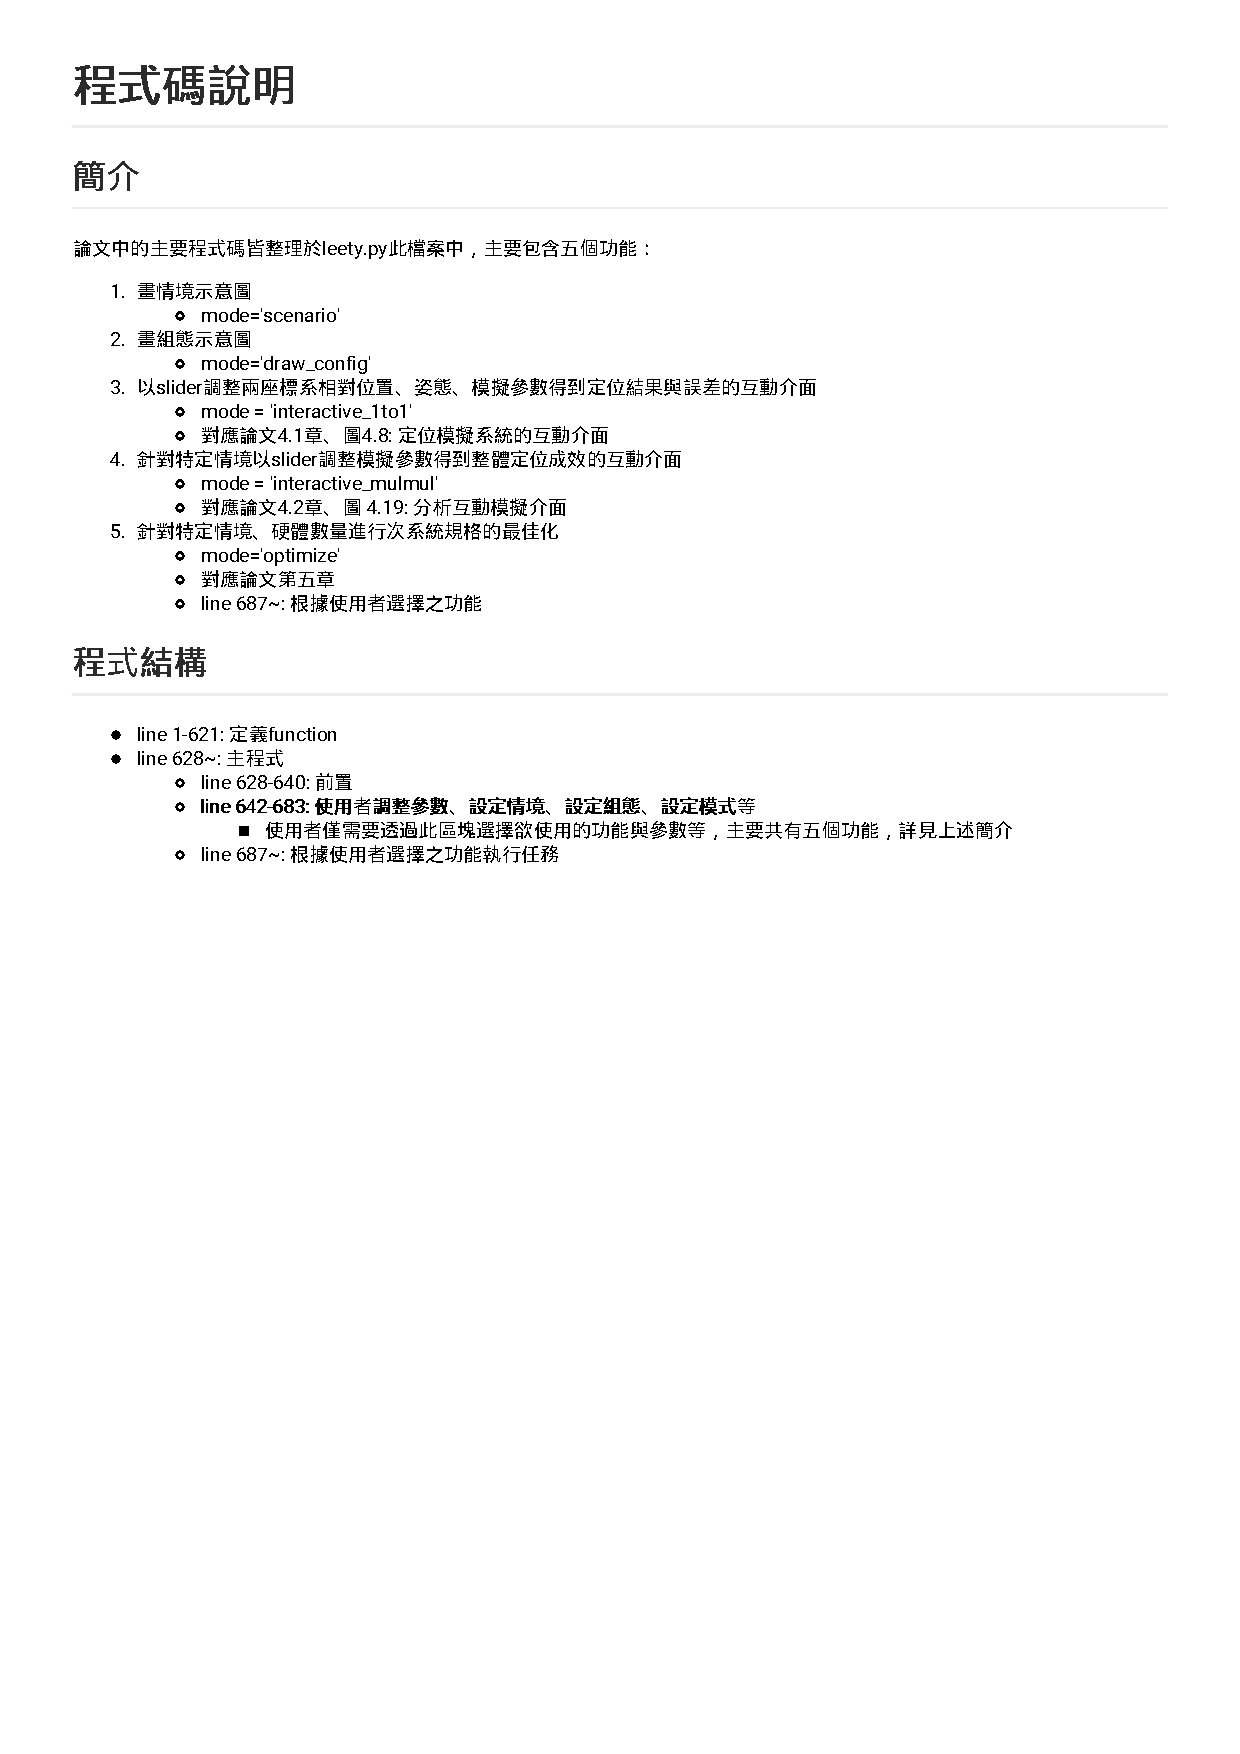
\includegraphics[width=22cm]{ReadMe.pdf}
%or %chapter cite  == \include
%\chapter{附錄:程式碼說明}

\hspace*{-3cm}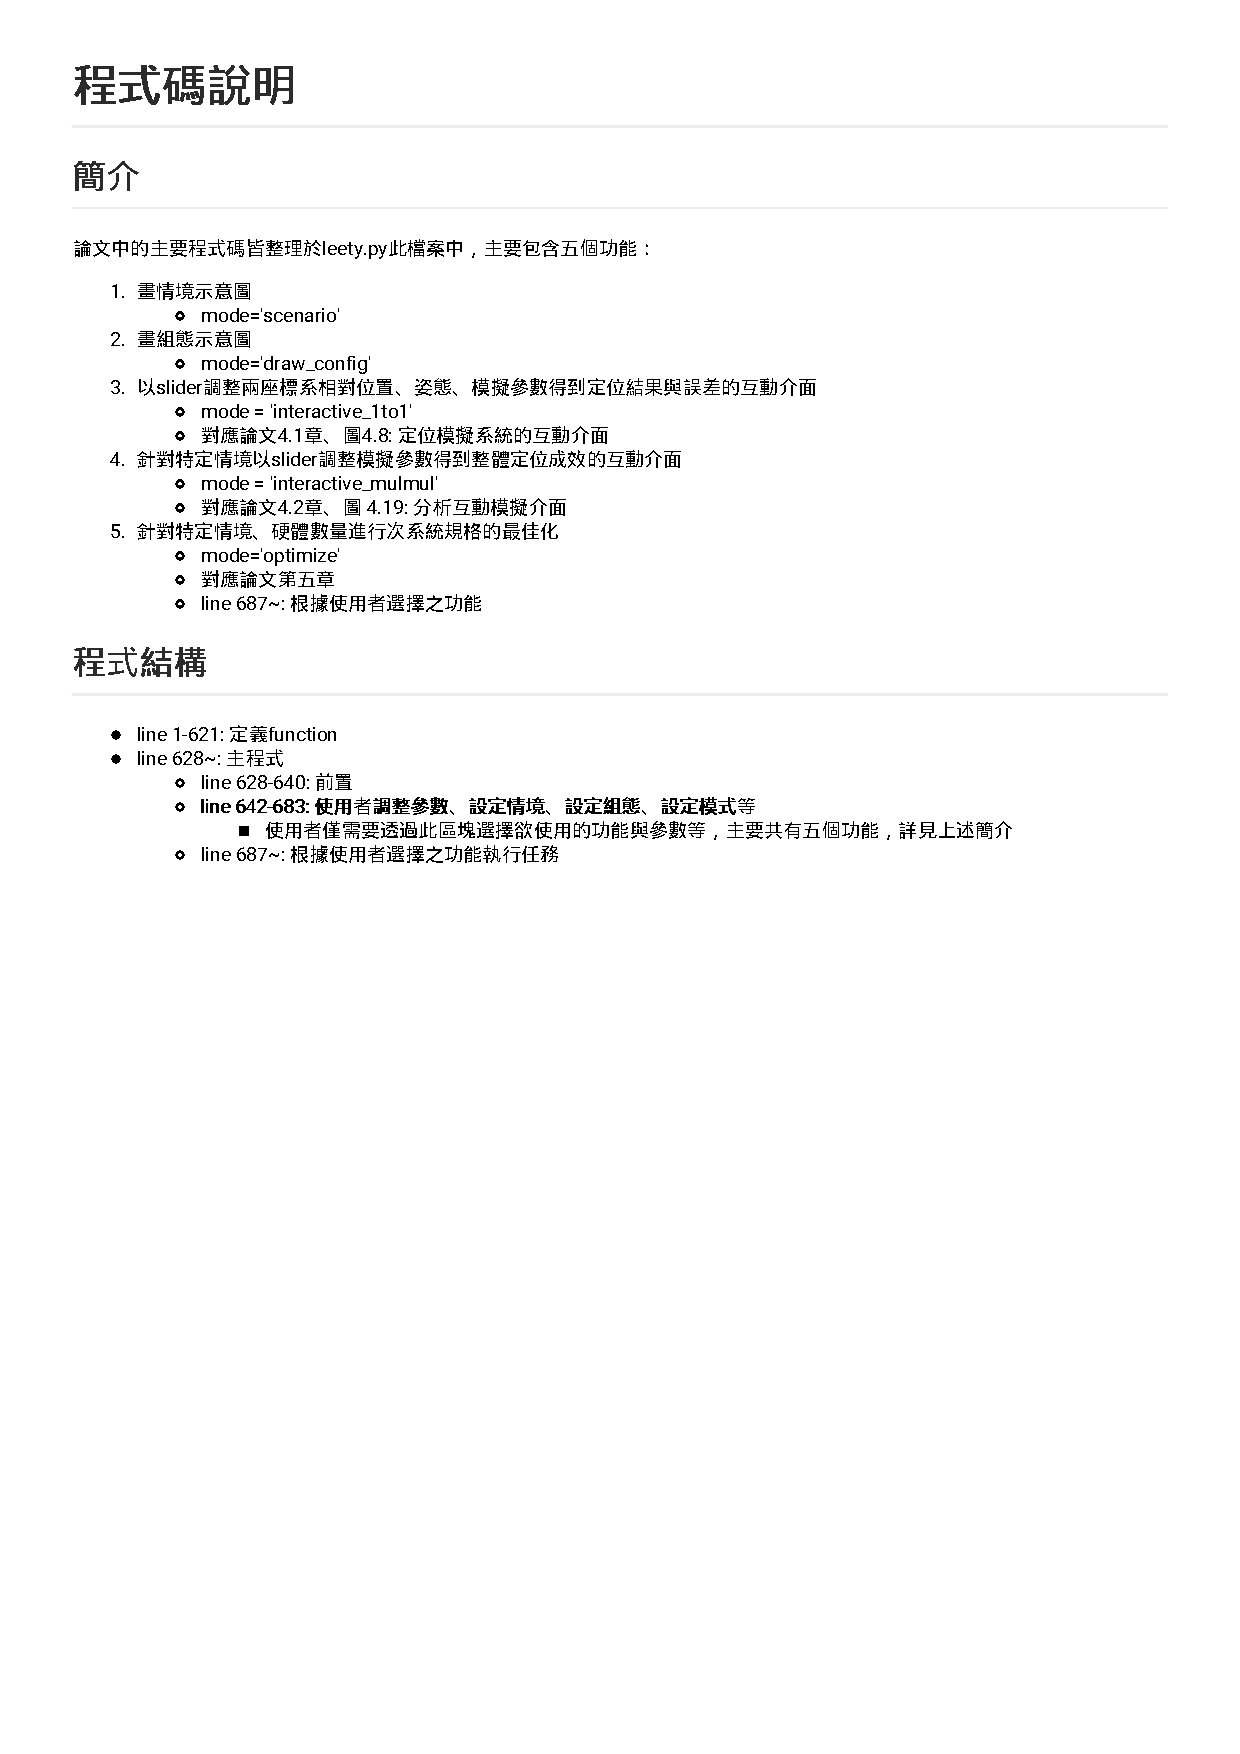
\includegraphics[width=22cm]{ReadMe.pdf}
    \end{verbatim}
    在章節檔\texttt{AppendixA.tex}裡,開頭打
    \begin{verbatim}
\chapter{First appendix title}
    \end{verbatim}
    即可,以此類推。    
        \item 系上規定論文圖表須全部放到最後獨立出來的章節,且章節不出現在目錄中:\\
    在\href{run:./thesis.tex}{thesis.tex}裡,依需求選擇input或include,刪去\texttt{\%}符號來輸入圖表章節
    \begin{verbatim}    
%----------- Input your Figure chapter here  -----------
%\input{EndFigTab} 
%chapter cite  == \include
%\include{EndFigTab}
    \end{verbatim}
    在章節檔\href{run:./EndFigTab.tex}{EndFigTab.tex}裡有範例和說明可供參考,要注意正文的圖表和附錄的圖表要分清楚,即在\href{run:./EndFigTab.tex}{EndFigTab.tex}內
    \begin{verbatim}    
\renewcommand{\thefigure}{\arabic{chapter}.\arabic{figure}} 
\renewcommand{\thetable}{\arabic{chapter}.\arabic{table}} 
%--- Input your main figures and tables here  ---
    \end{verbatim}
    這幾行之後章節計數器格式已切換為1\dots 9,放正文的圖表 ,
     \begin{verbatim}    
\renewcommand{\thefigure}{\Alph{chapter}.\arabic{figure}} 
\renewcommand{\thetable}{\Alph{chapter}.\arabic{table}}
%--- Input your appendix figures and tables here  ---
    \end{verbatim}
    這幾行之後章節計數器格式已切換為A\dots Z,放附錄的圖表。另外要取消圖表的浮動功能,才能讓圖表按照指令出現順序排好,即把平常使用的圖表指令
    \begin{verbatim}    
\begin{figure}[htb]
...
\begin{table}[htb]
    \end{verbatim}
    改成
     \begin{verbatim}    
\begin{figure}[!]
...
\begin{table}[!]
    \end{verbatim}
    剩下的只要注意章節圖表的計數器設定即可。\texttt{\textbackslash ref}和\texttt{\textbackslash label}指令可以在此圖表章節與正文章節使用。
     \item 如果我想要修改margin(文字邊界)的話,可以從哪裡下手呢?\\
     請打開\href{run:./ntu.sty}{ntu.sty}修改下面這行的上下左右參數即可:
    \begin{verbatim}
\RequirePackage[top=3cm,left=3cm,bottom=2cm,right=3cm]{geometry}
    \end{verbatim}
    \item 我想引用Twomey (1974): Pollution and planetary albedo這篇論文,如何用\texttt{\textbackslash cite}引用它的時候在內文顯示Twomey (1974) [編號] ?\\
    建議使用natbib套件,參考資料如下:\\
    \href{http://en.wikibooks.org/wiki/LaTeX/Bibliography_Management}{LaTeX/Bibliography Management}\\
    \href{http://nodonn.tipido.net/bibstyle.php}{Overview of Bibtex-Styles}\\
    \href{http://merkel.zoneo.net/Latex/natbib.php}{Reference sheet for natbib usage }\
 \item \XeTeX\ :\\
    此範本中文字體使用\XeTeX\ 轉換,細節請參考\href{http://www.hitripod.com/blog/}{Hitripod}寫的\href{http://www.hitripod.com/blog/2011/04/xetex-chinese-font-cjk-latex/}{ 
XeTeX:解決 LaTeX 惱人的中文字型問題}。
 \item 如何輸入英文`單引號'和``雙引號''以及不同長度的破折號?\\
        可以參考\href{run:./latex123.pdf}{李果正-大家來學\LaTeX}第17頁針對標點符號的遊戲規則,範例如下,輸入以下指令:\\
        \begin{verbatim}
`單引號'\\
``雙引號''\\
-hyphen\\
--en-dash\\
---em-dash\\
        \end{verbatim} 
        則顯示:\\
       `單引號'\\
        ``雙引號''\\
        -hyphen\\
        --en-dash\\
        ---em-dash\\
    \end{enumerate} 
    \end{enumerate} 
               

%----------- Have a fractal fern? -----------
%\begin{pspicture}
%\psFern[scale=30,maxIter=100000,linecolor=Green]
%\end{pspicture}

 \end{acknowledgementsCH}
\begin{abstractCH}

  隨著科技與物連網的發展,各領域對於量測資訊的需求大量增加,其中相對位置的資訊實為重要。然而,現今室內定位仍仰賴多個參考點進行定位,缺乏僅以「可攜式單位」達到兩物體之間三維定位的方法。因此,我們由探討不同的室內定位方法開始,根據以上需求將研究重點聚焦在光波段中發光二極體(Light Emitting Diode,簡稱LED)與光電二極體(Photodiode,簡稱PD)的定位方法,此方法有達到兩單位之間三維定位的潛力,但現今文獻中對使用情境與系統設計的限制仍許多,大多需限制接收與發射平面平行且僅能達到二維定位,除此之外也會對硬體進行限制。因此,本研究針對LED與PD的定位方法,建立一個可以不限制接收與發射平面平行的三維定位演算法,也不限制硬體的朗博次方(Lambertian Order)、硬體數量以及各硬體的擺放指向,使系統具有根據不同情境進行改變與設計的能力,改善此領域中對系統設計以及使用情境較多的限制。建立演算法後,本研究由該演算法建立一模擬環境與系統成效的量化方式,於模擬環境中,我們可以評估各系統設計下的定位效能,並透過改變不同的系統設計、使用情境與應用範圍(Region of Interest)、以及誤差參數,來觀察以及探討各參數對系統成效的影響。除此之外,本研究針對不同的使用情境,將系統設計作為變數進行最佳化,可將該最佳系統設計作為實際硬體系統搭建的參考。總結來說,本研究提供一僅利用兩單位進行三維定位的定位演算法,並建立一模擬環境,讓使用者得以在不浪費硬體搭建的成本下對系統設計進行分析與評估,也可以針對特定的使用情境進行系統設計的最佳化,在硬體系統搭建前達到有效的評估。

  % 此定位演算法對

  \vspace{1cm}
  \noindent \textbf{關鍵字:室內定位、光定位、發光二極體、光電二極體、定位演算法、最佳化}

\end{abstractCH}

\doublespacing
\begin{abstractEN}

    With the development of IoT, the demand of sensors and data,especially positioning information, has increased drastically. Nowadays, indoor positioning systems mostly use multiple reference points in order to obtain position information. There is no efficient way to get 3-dimensional relative position with only two portable unit. Therefore, we start from introducing different positioning methods and techniques. According to the aforementioned demand, we focused on the positioning technique of using LEDs and photodiodes. Although this technique has the potential fulfill the needs, the majority of nowadays research have restricted usage scenario and system design. Particulary, they could only obtain 2-dimensional position while restricting transmitting and receiving planes to be parralel. As a result, we developed a positioning algorithm which can abtain 3-dimensional position without planes parralel assumption. Other than this, Lambertian order, hardware amound and hardware placing direction are not constrained either, which means the system has the ability to adjust with respect to different scenario. With this positioing algorithm, we further set up a simulation environment and a method to quantify system performance. In the simulation environment, we can evaluate system performance with different system design in different scenario. By evaluation method, the influence of each system design variable and noise simulation variable can be discussed. Aside from evaluation, we also proposed a optimization method to take system design as variable and in specific scenario. Overall, we proposed a 3-dimensional positioning algorithm without parallel planes assumption while considering Lambertian order, hardware amount and placing orientation as variable. Except for positioning algorithm, the simulation environment and optimization method provide users a very a guide to construct the hardware system. 

    \vspace{1cm}
    \noindent \textbf{Key Words:Indoor Positioning, Light Positioning, Light-Emitting-Diode, Photodiode, Positioning Algorithm, Lambertian Order}

\end{abstractEN}


%\doublespacing
\onehalfspacing
\tableofcontents
\listoffigures
\listoftables

\mainmatter

%\doublespacing

%----------- Include/Input your thesis here -----------
%normal cite == \input
\chapter{}
%\input{start}
%\input{THM}
%\input{EXP}
%\input{main}
%\input{conclusions}

%chapter cite  == \include
%\include{start}
%\include{introduction}
%\include{THM}
%\include{EXP}
%\include{main}
%\include{conclusions}


%----------- Input your appendix here  -----------
\appendix
\titlecontents{chapter}[0em]{\fontsize{12}{18}\selectfont}
  {\hspace{3.5em}\contentslabel[附錄\,\thecontentslabel]{3.5em}}
  {}{\hspace{0.5em}\titlerule*{.}\contentspage}

\titleformat{\chapter}[display]
	{\bf\Large}
	{\filleft 附錄\,\thechapter}
	{1ex}
	{\huge\titlerule
	 \vspace{2ex}%
	 \filright}
	[\vspace{2ex}%
	 \titlerule]

\chapter{附錄:程式碼說明}

\hspace*{-3cm}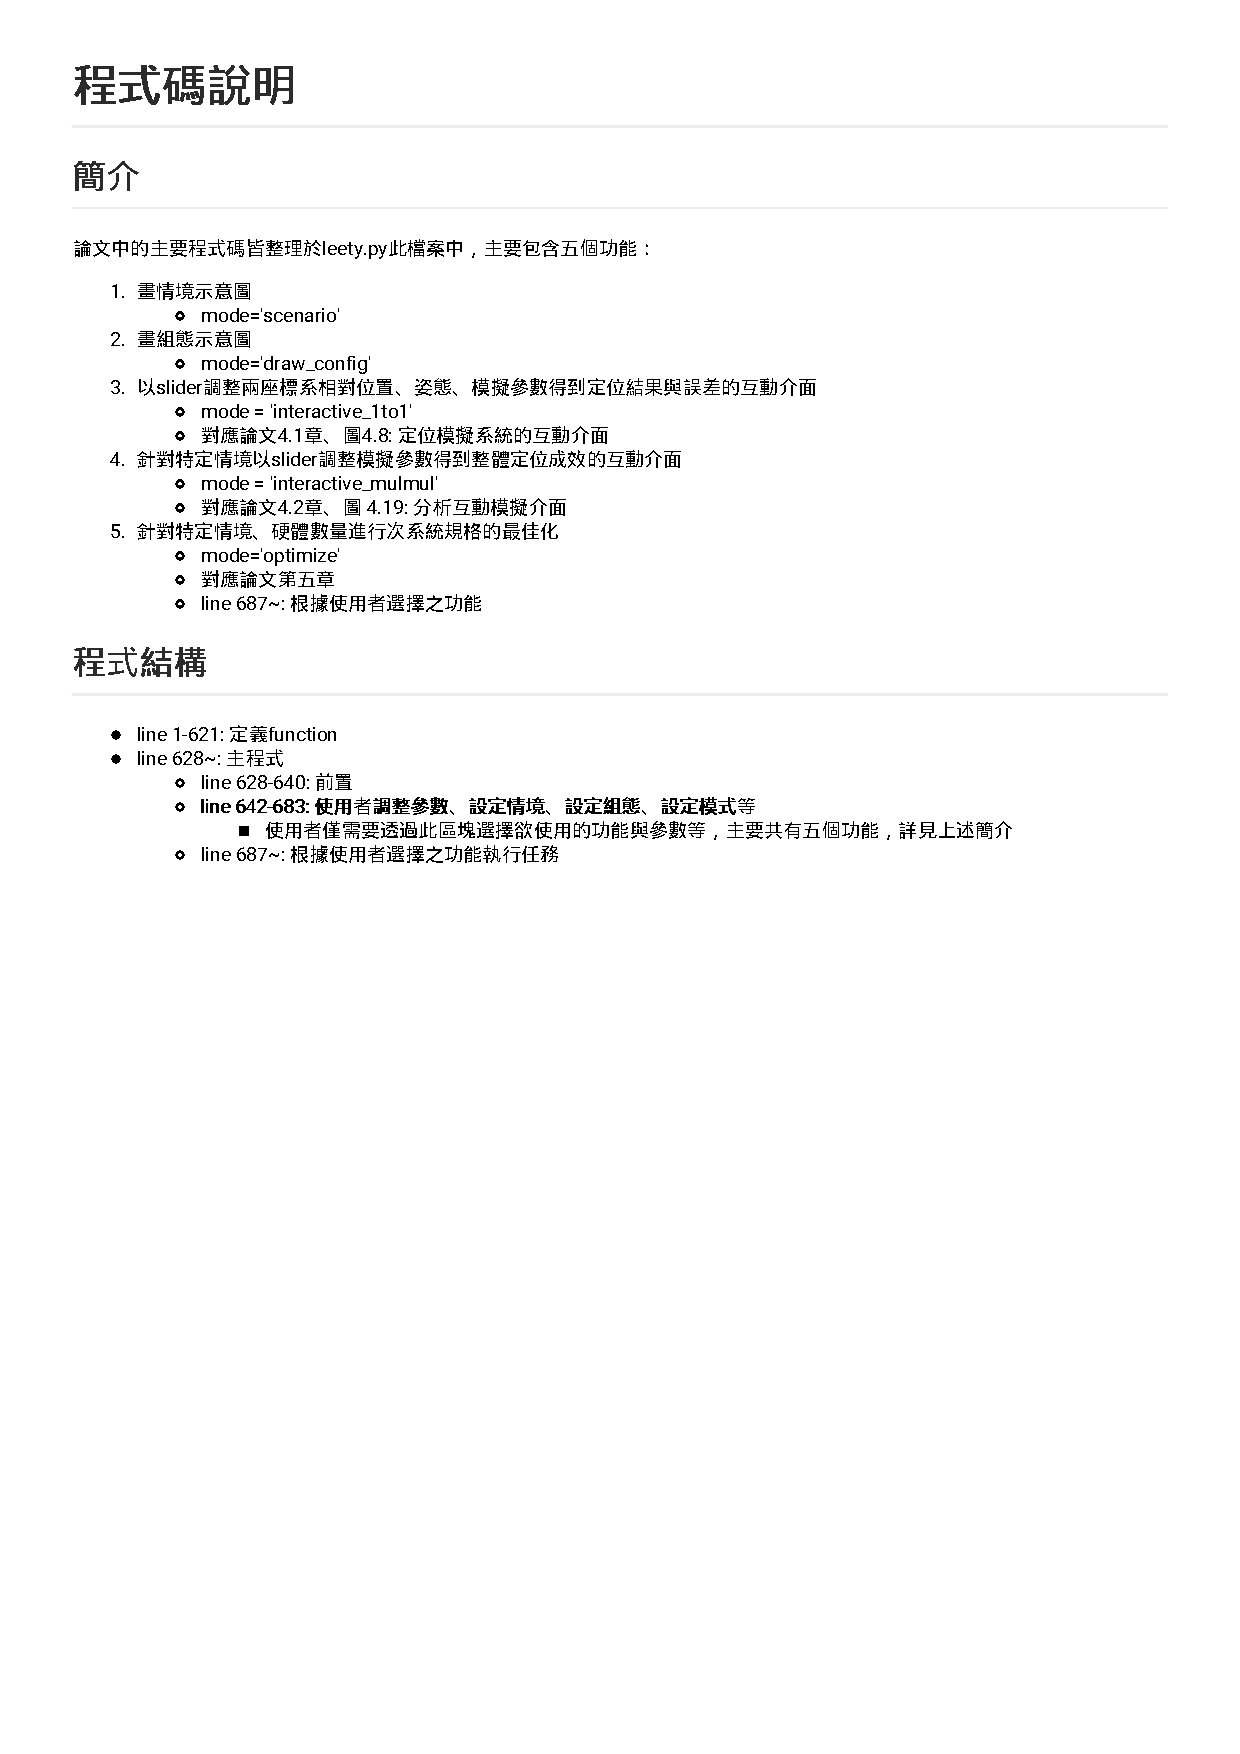
\includegraphics[width=22cm]{ReadMe.pdf} 



\backmatter


%---------- Input your reference here ---------
\bibliographystyle{ieeetr}
\addcontentsline{toc}{chapter}{\bibname}
\bibliography{thesisbib}

%----------- Input your Figure chapter here  -----------
%\input{EndFigTab} 
%chapter cite  == \include
%\include{EndFigTab}

\end{document}
